% Title : Project-II
% Author: Bhishan Poudel
% Date  : Dec 9, 2015 Sat

\documentclass[11pt,a4paper,english]{article}
\usepackage{babel}
\usepackage{amsmath}
\usepackage{amssymb}
\usepackage{graphicx,subfigure}
\usepackage[export]{adjustbox}    % for positioning figure
\usepackage{textcomp}
\usepackage{fixltx2e}
\usepackage[usenames,dvipsnames,svgnames,table]{xcolor}

% some useful newcommands
\newcommand{\nl}{\nonumber \\}
\newcommand{\no}{\nonumber}
\newcommand{\ul}{\underline}
\newcommand{\ol}{\overline}

%some useful newcommands
\newcommand{\beq}{\begin{equation}}
\newcommand{\eeq}{\end{equation}}
\newcommand{\bfig}{\begin{figure}}
\newcommand{\efig}{\end{figure}}
\newcommand{\beqa}{\begin{eqnarray}}
\newcommand{\eeqa}{\end{eqnarray}}
\newcommand{\beqan}{\begin{eqnarray*}}
\newcommand{\eeqan}{\end{eqnarray*}}
\newcommand{\ba}{\begin{array}}
\newcommand{\ea}{\end{array}}
\newcommand{\ben}{\begin{enumerate}}
\newcommand{\een}{\end{enumerate}}
\newcommand{\bfl}{\begin{flushleft}}
\newcommand{\efl}{\end{flushleft}}
\newcommand{\btab}{\begin{tabular}}
\newcommand{\etab}{\end{tabular}}
\newcommand{\bit}{\begin{itemize}}
\newcommand{\eit}{\end{itemize}}
\newcommand{\bdes}{\begin{description}}
\newcommand{\edes}{\end{description}}
\newcommand{\bdm}{\begin{equation}}
\newcommand{\edm}{\end{equation}}
\newcommand {\IR} [1]{\textcolor{red}{#1}}

% for listing
\usepackage{enumitem}
\usepackage[ampersand]{easylist}
\ListProperties(Hide=100, Hang=true, Progressive=3ex, Style*=-- ,
Style2*=$\bullet$ ,Style3*=$\circ$ ,Style4*=\tiny$\blacksquare$ )    % for easylist
\newcommand{\begl}{\begin{easylist}}
\newcommand{\eegl}{\end{easylist}}

% for hyperlink
\usepackage{hyperref}             % for hyperlink
\hypersetup{
    colorlinks=true,
    linkcolor=blue,
    filecolor=magenta,      
    urlcolor=cyan,    
    bookmarks=true
    }


% Creating Title for the assessment

\title{Project II : Bound States in Momentum Space}
\author{Bhishan Poudel}
\date{Dec 9,2015}

% to avoid indentation in paragraphs
\usepackage[parfill]{parskip}

% begin of document
\begin{document}
\maketitle
\tableofcontents
\listoffigures
\clearpage

%%%%%%%%%%%%%%%%%%%%%%%%%%%%%%%%%%%%%%%%%%%%%%%%%%%%%%%%%%%%%%%%%%%%%%%%%%%%%%%%%%%%%%%%%%%%%%%%%%%%%

\section{Qn 1: Legendre Polynomials }
In this part I wrote a code to calculate the legendre polynomials of orders from
$0$ to $8$ . I used the recursion formula:\\
\begin{equation}
(n+1) P_{n+1}(x) = (2n+1) x P_n(x) - nP_{n-1}(x)
\end{equation}
 to calculate the polynomials.
The calculated polynomials are accurate up to seven significant digits.
I used Wolfram Alpha online to check the accuracy of the legendre polynomials.
For example I took the value $x=0.8$ and compared the values.
%%==============================================================================
\begin{center}
	\begin{tabular}{llll}
		 n&x  & calculated p(n,0.8)  & Wolfram p(n,0.8) \\
		 0&0.8  &1.0000000  &1  \\
		 1&0.8  &0.8000000  &0.8  \\
		 2&0.8  &0.4600000  &0.46  \\
		 3&0.8  &0.0800000  &0.08  \\
		 4&0.8  &-0.2330000  &-0.233  \\
		 5&0.8  &-0.3995200  &-0.39952  \\
		 6&0.8  &-0.3917960  &-0.391796  \\
		 7&0.8  &-0.2396512  &-0.2396512  \\
		 8&0.8  &-0.0166553  &-0.0166553  \\
	\end{tabular}
	\label{tab:}
\end{center}
%%==============================================================================
I also checked the accuracy of my results by comparing the result of integral:\\
\begin{equation}
\int_{-1}^{1} \!\! P_{n}^2(x)\,dx
\end{equation}
obtained from my code to find polynomials with the orthogonality relation:\\
\begin{equation}
\frac{2}{2n+1} 
\end{equation}
The values are true up to seven significant figures, which we can see in the file 
`$legendre\_compare.dat$'

	The solution directory is :\\
	\begin{verbatim}
	location             : Pr2/Part1
	source code          : Legendre_Polynomials.f90 and legendre_compare.f90
	plots                : legendre_polynomials.eps
	datafiles            : legendre_polynomials.dat and legendre_compare.dat
	provided subroutines : gauleg.f90 
	\end{verbatim}
	
	    The figures are shown below:\\
    %%%% including figure %%%%%%%%%%%%%%%%%%
	\begin{figure}[h!]
	\centering
	\includegraphics [scale=0.6]{figures/legendre_polynomials.eps}
	\caption{Legendre Polynomials }
	\end{figure}
	\clearpage
	%%%%%%%%%%%%%%%%%%%%%%%%%%%%%%%%%%%%%%%	
	
\section{Qn 2: Partial Waves Potentials }
	
	
	In this Qn I calculated the partial wave potentials $v_0$, $v_2$, $v_4$.
	Where, $v_l$ is the partial wave potential given by:\\
	
	\begin{equation}
	v_l(q,q') = 2\pi \int_{-1}^{1} \!\! P_{l}(cos\theta) V(q,q')\,d(cos\theta)
	\end{equation}
	Where, $V(q,q')$ is the interaction potential between neutron and proton given
	in the question. $P_l$ is the Legendre polynomial of order $l$ and $q$,$q'$ are
	relative momenta for the proton-neutron system.\\
	I plotted the two graphs for $v_0$,$v_2$,$v_4$ for constant value of $q'=0.5 fm^{-1}$
	and $q'=2.5 fm^{-1}$
	  
%%%%%%%%%%%%%%%%%%%%%
\begin{figure}[!ht]
\hfill
\subfigure[for $q'=0.5 fm^-1$]{\includegraphics[width=6cm]{figures/potentialA.eps}}
\hfill
\subfigure[for $q'=2.5 fm^-1$]{\includegraphics[width=6cm]{figures/potentialB.eps}}
\hfill
\caption{deuteron potentials for different $q'$ }
\end{figure}
%%%%%%%%%%%%%%%%%%%%%%%
	
\section{Qn 3: Schrodinger equation using matrix }
    The Unit analysis is presented at the end of this document.\\
    The solution algorithm is like this:\\
    First, I solved the momentum space Schrodinger equation for two
    (neutron and proton) of reduced mass $\mu=m/2$given by:\\
	\begin{equation}
	      \frac{q^2}{2\mu} \Psi_{nl}(q) \\
	    + \frac{2}{\pi} \int_{0}^{\infty} \!\! p^{''2} v_l(q,p') \Psi_{nl}(p')\,dp' \\
	 = E_n\Psi_{nl}(q)
	\end{equation}
	This is a second order differential equation. To solve this equation, first I
	wrote the integral equation as the matrix equation and calculated the determinant
	of the matrix using LAPACK algorithm DGEEV. Then I found the value of binding energy
	using condition that the values must be less than zero.
	I followed the process given in Morten Hjorth-Jensen Lecture Notes Fall 2007 Chapter
	12.8.
	
\section{Qn 4: Gauss-Legendre mapping for the integration }
    To solve the integral part of $v_l(q,q')$ I used the Gauss-Legendre method.
    I used the given subroutine `gauleg' to solve the integral.
    To solve an integral first of all we have to convert it to summation.\\
    \begin{equation}
    \int_{a}^{b} \!\! f(x)\,dx = \sum_{i=1}^{N} w_i f(x_i) \\
    \end{equation}
    Where, N is Number of mess points, $w_i$ are weights, $x_i$ are points and
    $f(x_i)$ is the function to integrate.
    Here, also I have to use the mapping to $(0,\infty)$. So i used 
    following mapping:\\
    \begin{eqnarray}
    p_i &=& tan\frac{\pi}{4}(1+x_i)\\
    w_i &=& \frac{\pi}{4} \frac{w_i}{cos^2(\frac{\pi}{4}(1+x_i))}
    \end{eqnarray}
    
    
\section{Qn 5: Binding energy and errors }
    In this part I evaluated the binding energy of the deuteron.\\
    I used 50 number of gauss points to find the integral and the 
    final value of binding value obtained is -56.3 Mev.
    The source code is `pr2qn5.g90'

\section{Qn 6: Normalized ground state wavefunction }
    In this part I evaluated the normalized ground state wavefunction.
    The code is `pr2qn6.f90'. The plot is shown below:\\
%%%%%%%%%%%%%%%%%%%%%
\begin{figure}[!ht]
\hfill
\subfigure[given Va]{\includegraphics[width=6cm]{figures/wavefunction.eps}}
\hfill
\subfigure[smaller Va]{\includegraphics[width=6cm]{figures/wavefunctionNew.eps}}
\hfill
\caption{ground state wavefunctions at different parameter Va }
\end{figure}
%%%%%%%%%%%%%%%%%%%%%%%
    

\section{Qn 7: Variation of constant $V_A$ }
    Here, The potential of the deuteron depends on the parameter $V_A$, which gives
    the strength of the attraction between neutron and proton. I varied the value 
    of this parameter and got new potentials and wavefunction.

\section{Qn 8: New normalized ground state wavefunction }
    Here, for new value of $V_A$ I plotted the graph, which is shown in Qn 6.

\section{Qn 9: Expectation value of kinetic energy operator }
    In this part I calculated the expectation value of kinetic energy of the deuteron.
    For $V_A = 1085.3073 Mevfm$ I found $H_0=0.001Mev$.\\
    For $V_A = 985.3073 Mevfm$ I found $H_0=6.9E-3Mev$.\\
    The total mass of free neutron and proton is different than that of deuteron.
    The mass difference is called mass deficit. This mass deficit in terms of
    energy is called binding energy of the deuteron. Its value is about 2.23 Mev.
    This means if we combine one proton and one neutron to form a deuteron, the gamma
    ray of energy 2.23 Mev will be emitted. Now, when we supply the gamma ray of 
    at least 2.23 Mev to a bound state deuteron, they will separate apart and will gain 
    kinetic energy. At any time,\\
    Total energy $=$ Kinetic energy $+$ Potential Energy\\
    is valid.
\section{Appendix}

    %%%% including figure %%%%%%%%%%%%%%%%%%
	\begin{figure}[!ht]
	\centering
	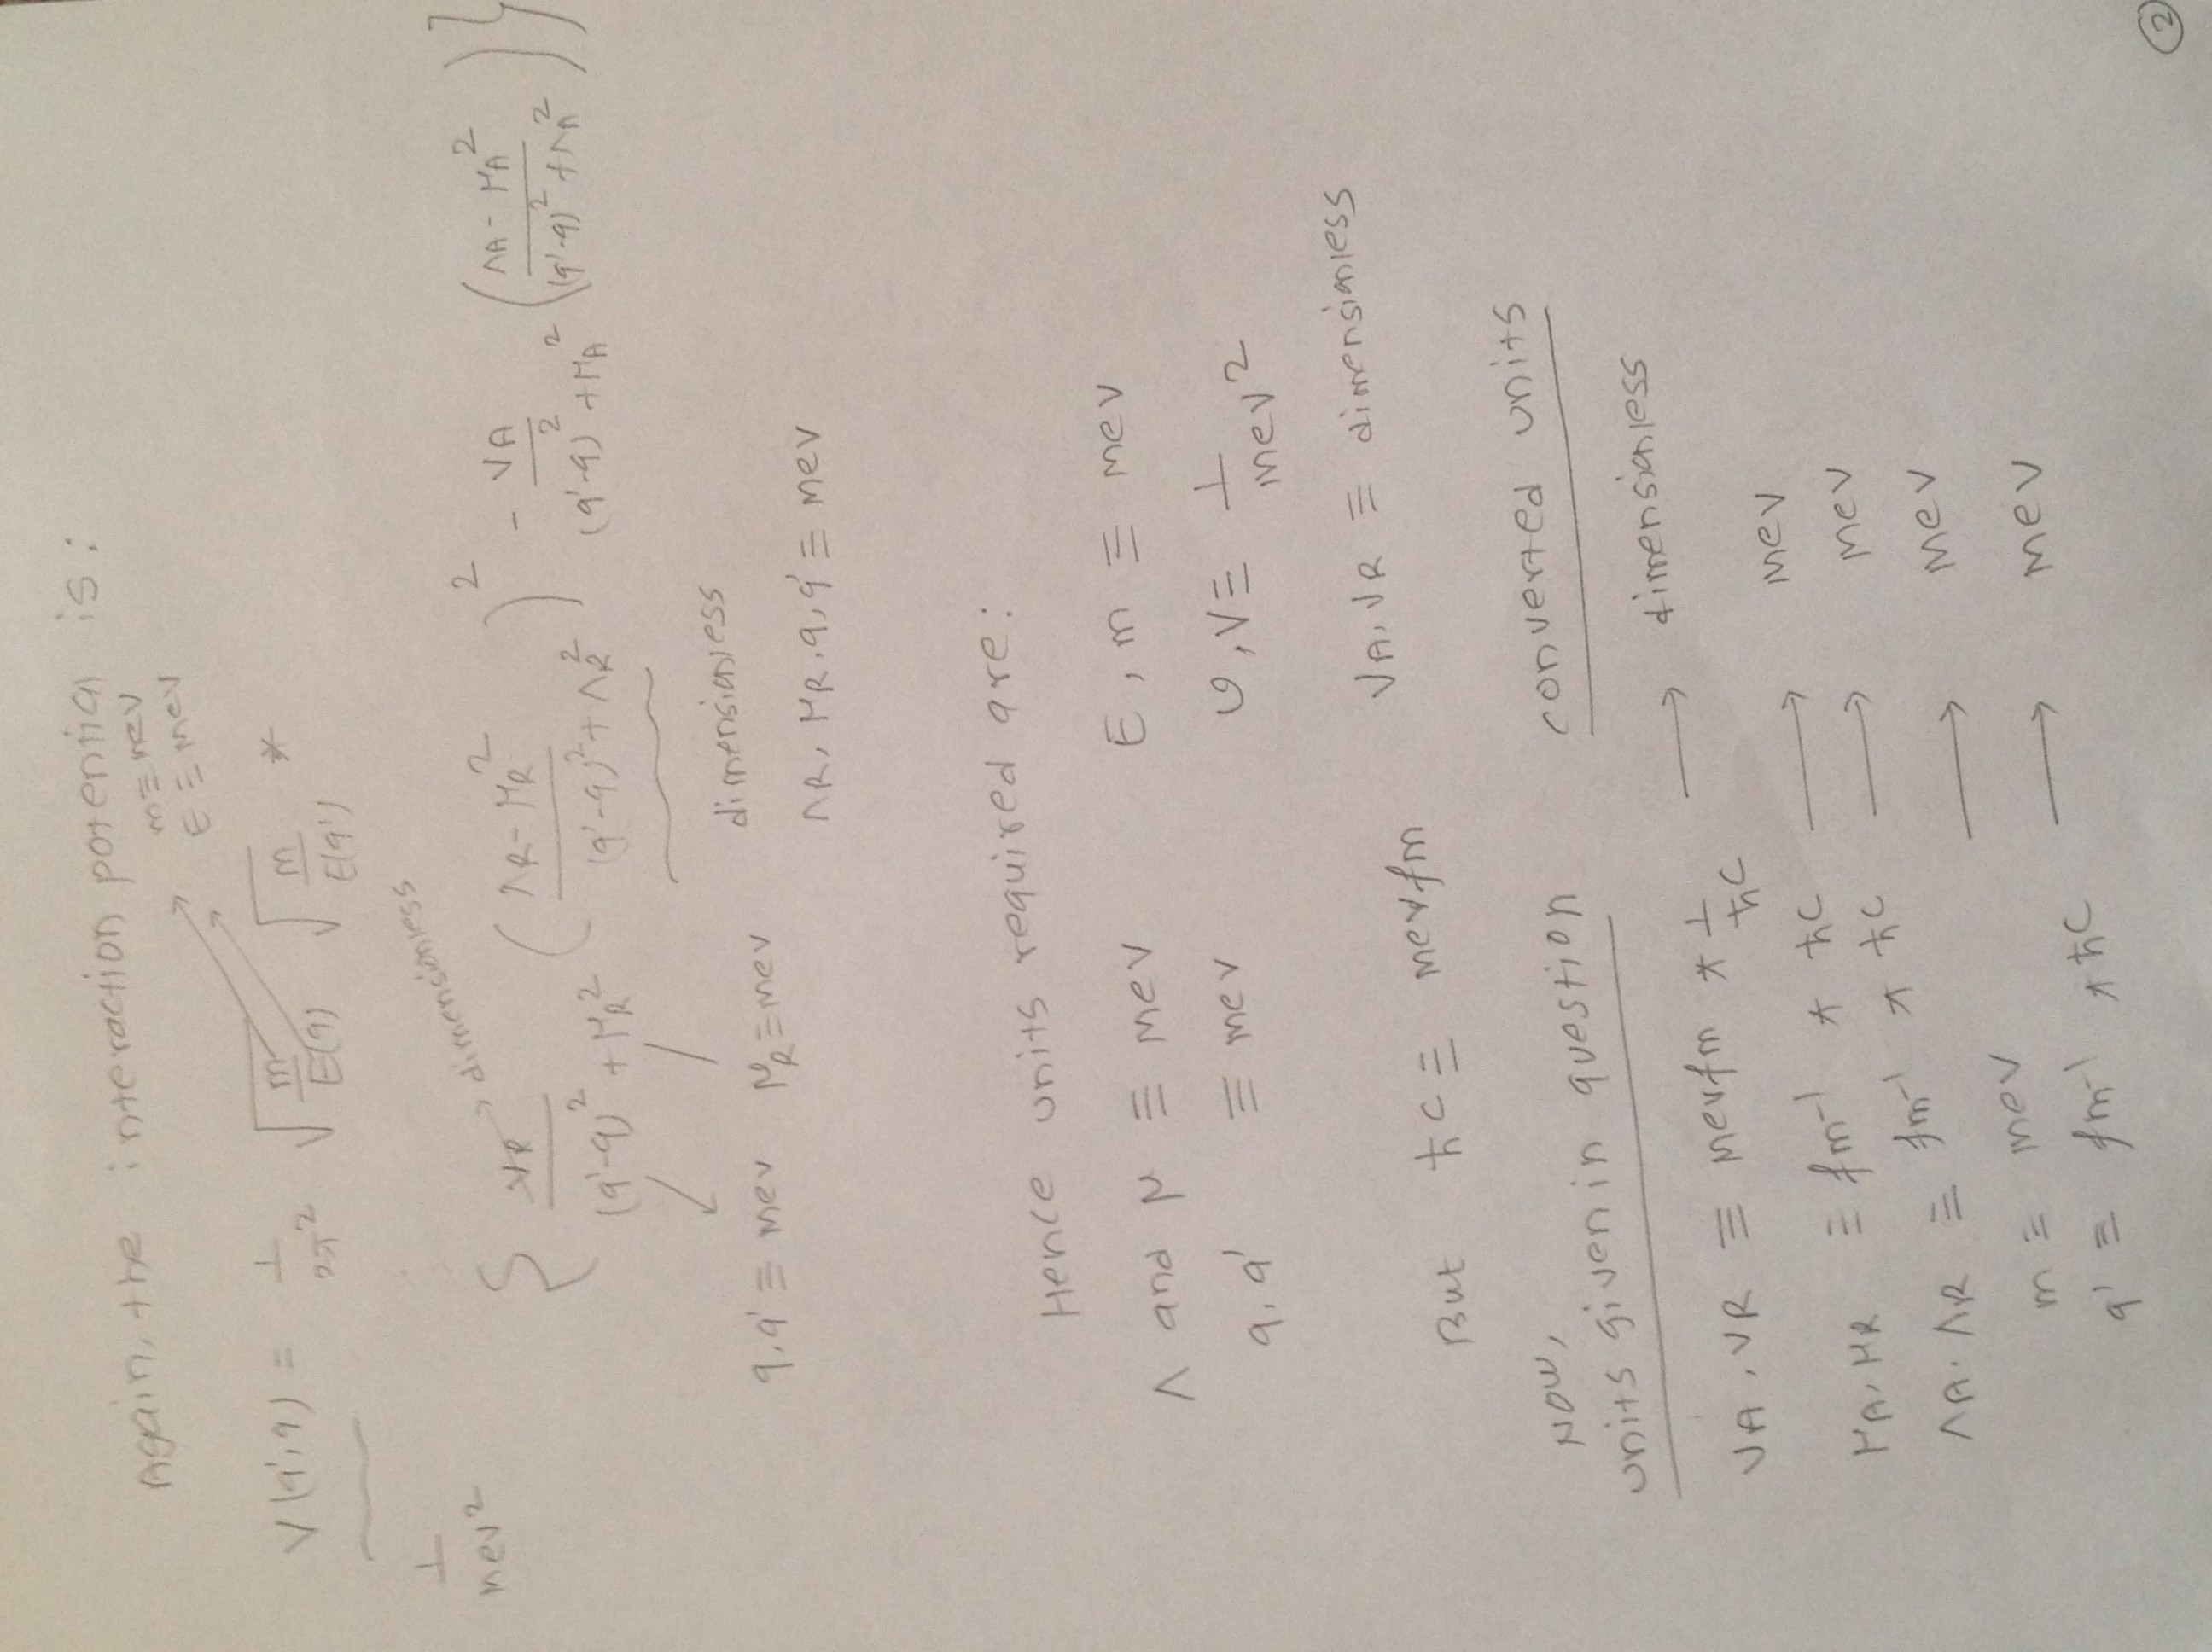
\includegraphics [scale=0.2,angle=270]{figures/1.eps}
	\caption{Unit Analysis page 1 }
	\end{figure}
	\clearpage
	%%%%%%%%%%%%%%%%%%%%%%%%%%%%%%%%%%%%%%%
	%%%% including figure %%%%%%%%%%%%%%%%%%
	\begin{figure}[!ht]
	\centering
	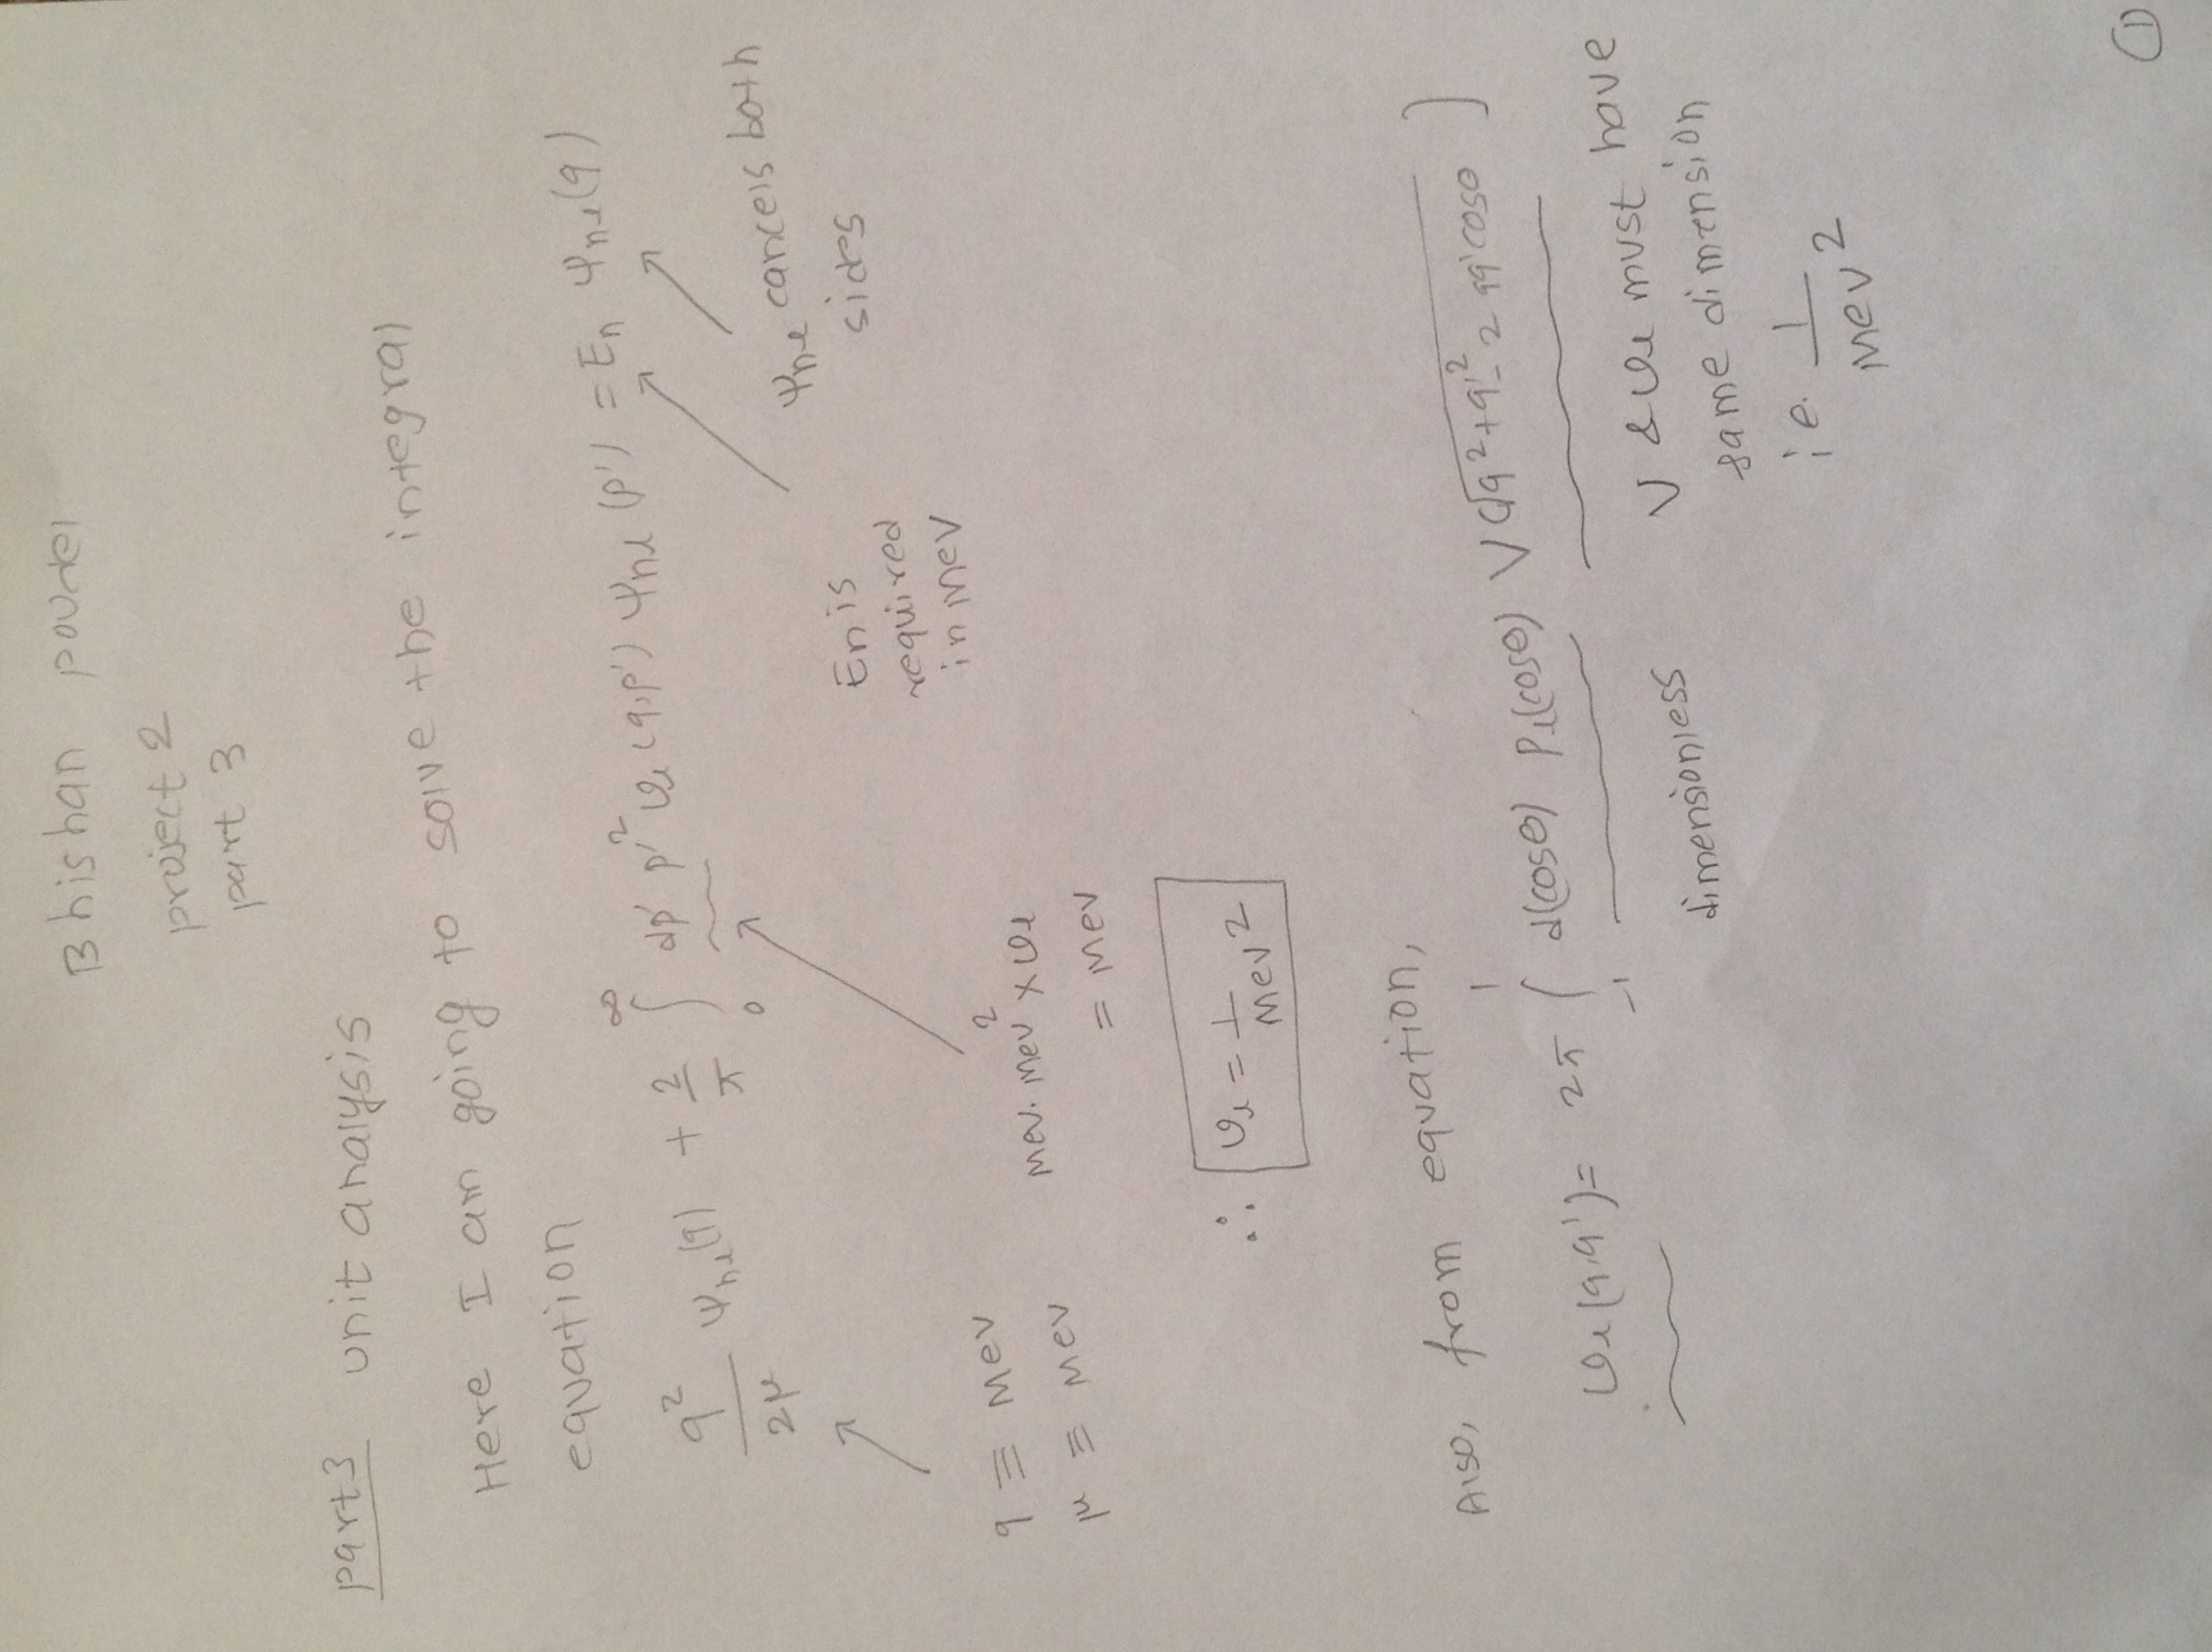
\includegraphics [scale=0.2,angle=270]{figures/2.eps}
	\caption{Unit Analysis page 2 }
	\end{figure}
	%%%%%%%%%%%%%%%%%%%%%%%%%%%%%%%%%%%%%%%	

    

\end{document}

